\subsection{Runder Stab, einseitig eingespannt} \label{sec:auswertung_einseitig_rund}
Zunächst wurde wieder eine Masse gewählt und fünfmal gewogen,
wobei sich im Mittel eine Masse von \SI{352.42 \pm 0.12}{\gram} ergab.

\begin{table}
\centering
\caption{Wiederholte Messung des benutzten Gewichts.}
\begin{tabular}{S}
\toprule
$m \mathbin{/} \si{\gram}$ \\
\midrule
352.2 \\
352.5 \\
352.4 \\
352.5 \\
352.5 \\
\bottomrule
\end{tabular}
\end{table}


In \autoref{tab:durchbiegung2} sind die Durchbiegung ohne Last ($D_\text{0}$), unter Last ($D_\text{M}$) und die tatsächliche Durchbiegung ($D$) mit der Position der Messuhr ($x$) aufgelistet.

\begin{table}
\centering
\caption{Durchbiegung des runden Stabes nach $x$-Abstand.}
\label{tab:durchbiegung2}
% \sisetup{table-format=2.1}
\begin{tabular}{c c c c}
\toprule
$x \mathbin{/} \si{\centi\meter}$ &
$D_0 \mathbin{/} \si{\micro\meter}$ &
$D_\text{M} \mathbin{/} \si{\micro\meter}$ &
$D \mathbin{/} \si{\micro\meter}$ \\
\midrule
\expandableinput{build/table_einseitig_rund.tex}
\bottomrule
\end{tabular}
\end{table}

\FloatBarrier

Es wurde $D(x)$ gegen den Linearisierungsterm $Lx^2-\frac{x^3}{3}$ aufgetragen (siehe \autoref{fig:regression2})
und mithilfe von NumPy eine Regressionsgerade $D(x) = k_2 \cdot x + c_2$ berechnet.
Deren Parameter sind:
\begin{align*}
  k_2 &= \SI{0.001454 \pm 0.000030}{\meter\tothe{-2}} \\
  c_2 &= \SI{-0.0027 \pm 0.0016}{\milli\meter} \; .
\end{align*}

Das Flächenträgheitsmoment $\mathbf{I}$ lässt sich diesmal durch \autoref{eqn:I_rund} mit den Abmessungen aus \autoref{sec:abmessungen} bestimmen.
%
% Die Gewichtskraft $F_G = g \cdot m$ ist durch die Erdbeschleunigung und die zuvor bestimmte Masse gegeben.

Schließlich ist
\begin{equation*}
  E
  = \frac{F_G}{2 k_2 \mathbf{I}}
  % Welch unintuitive Schreibweise! :/
  = \SI[{scientific-notation = true, separate-uncertainty = true}]{1.013(022)e5}{\newton\per\square\milli\meter}
\end{equation*}
der gesuchte Elastizitätsmodul.

% Die Messunsicherheit des Elastizitätsmoduls lässt sich gemäß der Gaußschen Fehlerfortpflanzung nach
% \begin{equation*}
%   \symup{\Delta}E = \frac{\partial E}{\partial m} \cdot \symup{\Delta}m
% \end{equation*}
% berechnen.

\begin{figure}
  \centering
  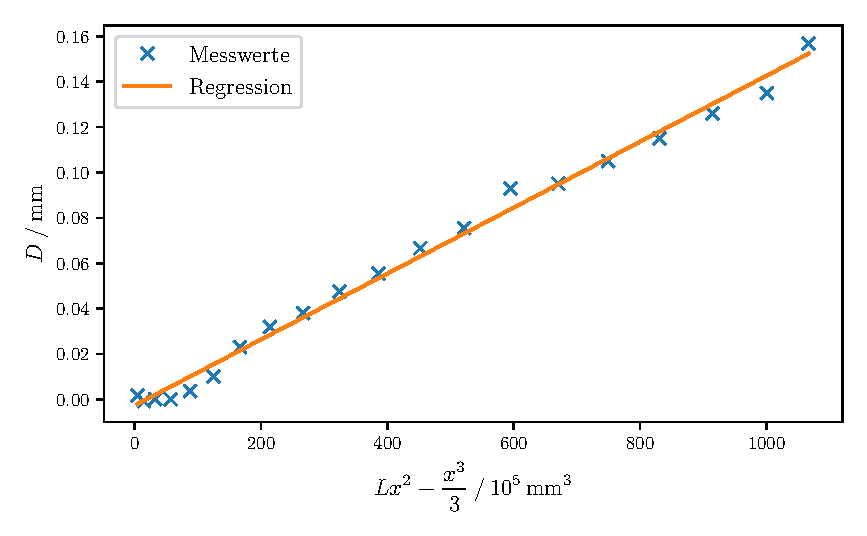
\includegraphics[scale=0.8]{build/plot_einseitig_rund.pdf}
  \caption{Durchbiegung eines einseitig eingespannten runden Stabes, aufgetragen gegen einen Linearisierungsterm.}
  \label{fig:regression2}
\end{figure}
